\documentclass[11pt]{article}

\usepackage[utf8]{inputenc}
\usepackage[T1]{fontenc}
\usepackage{lmodern}
\usepackage[margin=1in]{geometry}
\usepackage{amsmath,amssymb}
\usepackage{graphicx}
\usepackage{booktabs}
\usepackage{multirow}
\usepackage{xcolor}
\usepackage{tikz}
\usetikzlibrary{arrows.meta,positioning,fit,backgrounds}
\usepackage[numbers,sort&compress]{natbib}
\usepackage{url}
\usepackage[hidelinks]{hyperref}
\usepackage[capitalise,noabbrev]{cleveref}
\usepackage{caption}
\captionsetup{font=small,labelfont=bf}

\graphicspath{{../results/figures/npm_hi_n10k_contagion/}{../results/figures/}}

% Generated by `python -m src.paper_numbers` -- do not edit by hand.
\providecommand{\pending}{\textbf{[pending]}}
\newcommand{\CalOneBeta}{0.02}
\newcommand{\CalOneBetaM}{0.02}
\newcommand{\CalOneBetaMRange}{[0.005, 0.100]}
\newcommand{\CalOneBetaRange}{[0.010, 0.050]}
\newcommand{\CalOneCap}{20}
\newcommand{\CalOneDetect}{24}
\newcommand{\CalOneGamma}{0.10}
\newcommand{\CalOnePmajor}{65\%}
\newcommand{\CalOneShare}{76\%}
\newcommand{\CalOneSizeRange}{65--7{,}192}
\newcommand{\CalOneTninety}{41.5}
\newcommand{\CalTwoBeta}{0.20}
\newcommand{\CalTwoBetaM}{0.10}
\newcommand{\CalTwoBetaMRange}{[0.020, 0.200]}
\newcommand{\CalTwoBetaRange}{[0.100, 0.300]}
\newcommand{\CalTwoCap}{100}
\newcommand{\CalTwoDetect}{0}
\newcommand{\CalTwoGamma}{0.05}
\newcommand{\CalTwoPmajor}{68\%}
\newcommand{\CalTwoShare}{77\%}
\newcommand{\CalTwoSizeRange}{6{,}750--8{,}654}
\newcommand{\CalTwoTninety}{14.0}
\newcommand{\FiveAlphaIn}{2.62}
\newcommand{\FiveAlphaOut}{2.30}
\newcommand{\FiveAssortOutIn}{-0.129}
\newcommand{\FiveE}{15{,}907}
\newcommand{\FiveHooks}{1.5\%}
\newcommand{\FiveLLRLognormalIn}{-2.38}
\newcommand{\FiveLLRLognormalOut}{-0.87}
\newcommand{\FiveLambdaW}{2.00}
\newcommand{\FiveLargestSCC}{5}
\newcommand{\FiveMaxCore}{9}
\newcommand{\FiveMaxReach}{761}
\newcommand{\FiveMeanReach}{28.6}
\newcommand{\FiveN}{5{,}000}
\newcommand{\FiveNontrivialSCC}{19}
\newcommand{\FivePLognormalIn}{0.017}
\newcommand{\FivePLognormalOut}{0.386}
\newcommand{\FiveProvenance}{19.0\%}
\newcommand{\FiveSemverCaret}{74.1\%}
\newcommand{\FiveSemverExact}{10.5\%}
\newcommand{\FiveSemverTilde}{7.8\%}
\newcommand{\FiveSemverWildcard}{7.6\%}
\newcommand{\FiveTauTheory}{0.500}
\newcommand{\FiveXminIn}{6}
\newcommand{\FiveXminOut}{6}
\newcommand{\FullAlphaIn}{2.48}
\newcommand{\FullAlphaOut}{1.97}
\newcommand{\FullAssortOutIn}{-0.051}
\newcommand{\FullE}{60{,}041}
\newcommand{\FullHooks}{0.9\%}
\newcommand{\FullLLRLognormalIn}{-1.37}
\newcommand{\FullLLRLognormalOut}{-5.09}
\newcommand{\FullLambdaW}{8.98}
\newcommand{\FullLargestSCC}{46}
\newcommand{\FullMaxCore}{81}
\newcommand{\FullMaxReach}{2{,}305}
\newcommand{\FullMeanReach}{81.1}
\newcommand{\FullN}{14{,}624}
\newcommand{\FullNontrivialSCC}{56}
\newcommand{\FullPLognormalIn}{0.171}
\newcommand{\FullPLognormalOut}{0.000}
\newcommand{\FullProvenance}{25.3\%}
\newcommand{\FullRaw}{14{,}660}
\newcommand{\FullSemverCaret}{68.9\%}
\newcommand{\FullSemverExact}{16.7\%}
\newcommand{\FullSemverTilde}{8.8\%}
\newcommand{\FullSemverWildcard}{5.6\%}
\newcommand{\FullTauTheory}{0.111}
\newcommand{\FullXminIn}{7}
\newcommand{\FullXminOut}{2}
\newcommand{\MainAlphaIn}{2.39}
\newcommand{\MainAlphaOut}{2.08}
\newcommand{\MainAssortOutIn}{-0.069}
\newcommand{\MainE}{43{,}233}
\newcommand{\MainHooks}{1.0\%}
\newcommand{\MainLLRLognormalIn}{-1.68}
\newcommand{\MainLLRLognormalOut}{-2.74}
\newcommand{\MainLambdaW}{4.92}
\newcommand{\MainLargestSCC}{22}
\newcommand{\MainMaxCore}{74}
\newcommand{\MainMaxReach}{1{,}456}
\newcommand{\MainMeanReach}{45.0}
\newcommand{\MainN}{10{,}000}
\newcommand{\MainNontrivialSCC}{47}
\newcommand{\MainPLognormalIn}{0.093}
\newcommand{\MainPLognormalOut}{0.006}
\newcommand{\MainProvenance}{21.5\%}
\newcommand{\MainSemverCaret}{71.2\%}
\newcommand{\MainSemverExact}{15.0\%}
\newcommand{\MainSemverTilde}{7.6\%}
\newcommand{\MainSemverWildcard}{6.2\%}
\newcommand{\MainTauTheory}{0.203}
\newcommand{\MainXminIn}{8}
\newcommand{\MainXminOut}{5}
\newcommand{\NSeeds}{4{,}686}
\newcommand{\RQOneDepOnlyBridge}{0.2\%}
\newcommand{\RQOneDepOnlyBridgeMaint}{0\%}
\newcommand{\RQOneDepOnlyBridgePmajor}{0\%}
\newcommand{\RQOneDepOnlyHub}{2.6\%}
\newcommand{\RQOneDepOnlyHubMaint}{0\%}
\newcommand{\RQOneDepOnlyHubPmajor}{11\%}
\newcommand{\RQOneDepOnlyLeaf}{0.0\%}
\newcommand{\RQOneDepOnlyLeafMaint}{0\%}
\newcommand{\RQOneDepOnlyLeafPmajor}{0\%}
\newcommand{\RQOneDepOnlyMid}{0.0\%}
\newcommand{\RQOneDepOnlyMidMaint}{0\%}
\newcommand{\RQOneDepOnlyMidPmajor}{0\%}
\newcommand{\RQOneShOneBridge}{48.7\%}
\newcommand{\RQOneShOneBridgeMaint}{78\%}
\newcommand{\RQOneShOneBridgePmajor}{95\%}
\newcommand{\RQOneShOneHub}{55.8\%}
\newcommand{\RQOneShOneHubMaint}{76\%}
\newcommand{\RQOneShOneHubPmajor}{100\%}
\newcommand{\RQOneShOneLeaf}{19.6\%}
\newcommand{\RQOneShOneLeafMaint}{70\%}
\newcommand{\RQOneShOneLeafPmajor}{40\%}
\newcommand{\RQOneShOneMid}{31.8\%}
\newcommand{\RQOneShOneMidMaint}{73\%}
\newcommand{\RQOneShOneMidPmajor}{63\%}
\newcommand{\RQOneShTwoBridge}{84.2\%}
\newcommand{\RQOneShTwoBridgeMaint}{73\%}
\newcommand{\RQOneShTwoBridgePmajor}{98\%}
\newcommand{\RQOneShTwoHub}{85.8\%}
\newcommand{\RQOneShTwoHubMaint}{73\%}
\newcommand{\RQOneShTwoHubPmajor}{100\%}
\newcommand{\RQOneShTwoLeaf}{55.4\%}
\newcommand{\RQOneShTwoLeafMaint}{74\%}
\newcommand{\RQOneShTwoLeafPmajor}{64\%}
\newcommand{\RQOneShTwoMid}{78.8\%}
\newcommand{\RQOneShTwoMidMaint}{73\%}
\newcommand{\RQOneShTwoMidPmajor}{92\%}
\newcommand{\RQOneSpecRefBridge}{0.8\%}
\newcommand{\RQOneSpecRefBridgeMaint}{0\%}
\newcommand{\RQOneSpecRefBridgePmajor}{0\%}
\newcommand{\RQOneSpecRefHub}{5.3\%}
\newcommand{\RQOneSpecRefHubMaint}{0\%}
\newcommand{\RQOneSpecRefHubPmajor}{46\%}
\newcommand{\RQOneSpecRefLeaf}{0.0\%}
\newcommand{\RQOneSpecRefLeafMaint}{0\%}
\newcommand{\RQOneSpecRefLeafPmajor}{0\%}
\newcommand{\RQOneSpecRefMid}{0.2\%}
\newcommand{\RQOneSpecRefMidMaint}{0\%}
\newcommand{\RQOneSpecRefMidPmajor}{0\%}
\newcommand{\RQThreeAcquaintanceFortyEight}{34\%}
\newcommand{\RQThreeAcquaintanceOne}{3\%}
\newcommand{\RQThreeAcquaintanceSix}{17\%}
\newcommand{\RQThreeAcquaintanceTwelve}{32\%}
\newcommand{\RQThreeAcquaintanceTwentyFour}{35\%}
\newcommand{\RQThreeBudget}{50}
\newcommand{\RQThreeBudgetPct}{0.5\%}
\newcommand{\RQThreeFirebreakBetweennessFortyEight}{26\%}
\newcommand{\RQThreeFirebreakBetweennessOne}{3\%}
\newcommand{\RQThreeFirebreakBetweennessSix}{13\%}
\newcommand{\RQThreeFirebreakBetweennessTwelve}{27\%}
\newcommand{\RQThreeFirebreakBetweennessTwentyFour}{29\%}
\newcommand{\RQThreeHubImmunizationFortyEight}{40\%}
\newcommand{\RQThreeHubImmunizationOne}{6\%}
\newcommand{\RQThreeHubImmunizationSix}{23\%}
\newcommand{\RQThreeHubImmunizationTwelve}{38\%}
\newcommand{\RQThreeHubImmunizationTwentyFour}{42\%}
\newcommand{\RQThreeHubPatchingFortyEight}{3\%}
\newcommand{\RQThreeHubPatchingOne}{100\%}
\newcommand{\RQThreeHubPatchingSix}{90\%}
\newcommand{\RQThreeHubPatchingTwelve}{52\%}
\newcommand{\RQThreeHubPatchingTwentyFour}{13\%}
\newcommand{\RQThreeNoneFortyEight}{68\%}
\newcommand{\RQThreeNoneOne}{47\%}
\newcommand{\RQThreeNoneSix}{48\%}
\newcommand{\RQThreeNoneTwelve}{49\%}
\newcommand{\RQThreeNoneTwentyFour}{55\%}
\newcommand{\RQThreeRandomPatchingFortyEight}{1\%}
\newcommand{\RQThreeRandomPatchingOne}{100\%}
\newcommand{\RQThreeRandomPatchingSix}{76\%}
\newcommand{\RQThreeRandomPatchingTwelve}{23\%}
\newcommand{\RQThreeRandomPatchingTwentyFour}{5\%}
\newcommand{\RQTwoBDone}{\textbf{[pending]}}
\newcommand{\RQTwoBetaSD}{0.279}
\newcommand{\RQTwoBetaSL}{0.514}
\newcommand{\RQTwoBetaSQ}{0.045}
\newcommand{\RQTwoCredCollapsed}{75\%}
\newcommand{\RQTwoGammaLow}{0.02}
\newcommand{\RQTwoLockFactor}{12}
\newcommand{\RQTwoScriptsFactor}{6}
\newcommand{\RQTwoTauTheory}{0.203}
\newcommand{\SensHubLeafMax}{\textbf{[pending]}}
\newcommand{\SensHubLeafMin}{\textbf{[pending]}}
\newcommand{\SensProactiveBest}{\textbf{[pending]}}
\newcommand{\SpamRemoved}{36}
\newcommand{\SynAlphaIn}{2.95}
\newcommand{\SynAlphaOut}{1.94}
\newcommand{\SynAssortOutIn}{-0.033}
\newcommand{\SynE}{3{,}927}
\newcommand{\SynHooks}{2.8\%}
\newcommand{\SynHubMean}{38.3\%}
\newcommand{\SynHubSD}{5.0\%}
\newcommand{\SynLLRLognormalIn}{-6.54}
\newcommand{\SynLLRLognormalOut}{-0.17}
\newcommand{\SynLambdaW}{0.00}
\newcommand{\SynLargestSCC}{1}
\newcommand{\SynLeafMean}{5.4\%}
\newcommand{\SynLeafSD}{2.8\%}
\newcommand{\SynMaxCore}{6}
\newcommand{\SynMaxReach}{1{,}999}
\newcommand{\SynMeanReach}{20.6}
\newcommand{\SynN}{2{,}000}
\newcommand{\SynNontrivialSCC}{0}
\newcommand{\SynPLognormalIn}{0.000}
\newcommand{\SynPLognormalOut}{0.865}
\newcommand{\SynProvenance}{4.5\%}
\newcommand{\SynRQThreeBest}{Hub immunization}
\newcommand{\SynRQThreeBestCount}{6/6}
\newcommand{\SynSeeds}{6}
\newcommand{\SynSemverCaret}{68.2\%}
\newcommand{\SynSemverExact}{17.9\%}
\newcommand{\SynSemverTilde}{10.8\%}
\newcommand{\SynSemverWildcard}{3.0\%}
\newcommand{\SynTauTheory}{$\infty$}
\newcommand{\SynXminIn}{2}
\newcommand{\SynXminOut}{2}
\newcommand{\ValOneCoMaint}{98\%}
\newcommand{\ValOneCoMaintNull}{49\%}
\newcommand{\ValOneDepLinked}{32\%}
\newcommand{\ValOneDepLinkedNull}{5\%}
\newcommand{\ValOneInFull}{2}
\newcommand{\ValOneInMain}{2}
\newcommand{\ValOneListed}{203}
\newcommand{\ValOneN}{189}
\newcommand{\ValTwoCoMaint}{95\%}
\newcommand{\ValTwoCoMaintNull}{69\%}
\newcommand{\ValTwoDepLinked}{23\%}
\newcommand{\ValTwoDepLinkedNull}{14\%}
\newcommand{\ValTwoInFull}{7}
\newcommand{\ValTwoInMain}{0}
\newcommand{\ValTwoListed}{795}
\newcommand{\ValTwoN}{732}


\newcommand{\Rinf}{R_\infty}
\newcommand{\pkg}[1]{\texttt{#1}}

\title{Super-Spreaders, Firebreaks and Stolen Tokens:\\
SIR Modelling of Self-Propagating Worms in the npm Dependency Network}
\author{Author names withheld for draft}
\date{Draft --- \today}

\begin{document}
\maketitle

\begin{abstract}
In September and November 2025 the self-propagating worms Shai-Hulud and Shai-Hulud~2.0 compromised
roughly \ValOneListed{} and \ValTwoListed{} npm packages. They did so by stealing maintainers' publish
tokens during package installation and republishing those maintainers' packages with an injected
install script. We model such worms as a two-channel SIR epidemic on the npm ecosystem.
\begin{itemize}
  \item \textbf{Dependency channel.} A compromised dependency exposes its dependents, weighted by how
        permissive each SemVer range is and by whether consumers block lifecycle scripts.
  \item \textbf{Credential channel.} A leaked token lets the worm republish up to a capped number of
        the owner's packages.
\end{itemize}

Our main data set is a \MainN-package graph built from the npm registry. It is the dependency closure
of the \NSeeds{} most-depended-upon packages, cleaned of a reward-farming spam ring.

\textbf{Calibration and validation.} With one tick equal to one hour, we calibrate transmission,
credential and patching rates to the observed plateau times and stolen-token share of both waves.
Against the real compromised-package lists, victims share a maintainer with another victim far more
often than random package sets do (\ValOneCoMaint{} vs.\ \ValOneCoMaintNull{} for wave~1, \ValTwoCoMaint{}
vs.\ \ValTwoCoMaintNull{} for wave~2). They are almost absent from the high-impact core.

\textbf{Findings.}
\begin{itemize}
  \item With dependencies alone, spread is bounded: outbreaks started at the most-depended-upon packages
        reach only \RQOneDepOnlyHub{} of the core, and leaf-started outbreaks fizzle.
  \item With the calibrated credential channel, even a leaf patient zero reaches \RQOneShOneLeaf{}
        (wave~1 parameters) to \RQOneShTwoLeaf{} (wave~2) of the core.
  \item Strict lockfiles and script blocking raise the dependency-channel epidemic threshold
        \RQTwoLockFactor$\times$ and \RQTwoScriptsFactor$\times$. With stealable tokens, however, the
        threshold in the dependency transmission rate collapses to the bottom of our grid.
  \item Reactive patching prevents almost all spread if the worm is detected within an hour, but only
        \RQThreeHubPatchingTwentyFour{} after a realistic 24-hour detection lag. Proactively immunizing
        the same number of high-degree packages still prevents \RQThreeHubImmunizationTwentyFour.
\end{itemize}
Credential hardening and proactive protection of central packages therefore matter more than dependency
pinning.
\end{abstract}

\section{Introduction}\label{sec:intro}

Modern JavaScript applications are assembled from hundreds of npm packages. Each package declares its
own dependencies through SemVer ranges, and package managers resolve and install these transitively.
This creates a dense, directed web of trust. A compromise of a single widely used package can reach a
large part of the ecosystem~\citep{zimmermann2019smallworld,kikas2017structure,decan2019empirical}.
The exposure is no longer hypothetical. Account takeovers and malicious maintainer handovers have
repeatedly delivered malware through trusted packages~\citep{npm2018eventstream,github2021uaparser,
aikido2025chalkdebug,ohm2020backstabber}.

In 2025 the threat changed qualitatively, as worms began to propagate themselves:
\begin{itemize}
  \item \textbf{Shai-Hulud} (September) ran a malicious script at install time. The script harvested
        npm publish tokens from developer machines and CI runners, then used each stolen token to
        republish up to \CalOneCap{} of the victim's own packages with the same payload
        injected~\citep{stepsecurity2025shaihulud,socket2025shaihulud,cisa2025npm}.
  \item \textbf{Shai-Hulud~2.0} (November) used a preinstall hook and raised the per-token cap to
        \CalTwoCap{} packages~\citep{wiz2025shaihulud2,datadog2025shaihulud2}.
\end{itemize}
Each newly infected package infected whoever installed it next. Spread was limited only by detection and
registry intervention. These incidents raise network-scientific questions that static vulnerability
reachability studies~\citep{decan2018vulnerabilities,liu2022demystifying,zerouali2022vulnerabilities}
cannot answer:
\begin{itemize}
  \item How do the topology of the dependency graph and the ownership structure of maintainer accounts
        jointly determine how far and how fast such a worm spreads?
  \item Which ecosystem-level defences change the epidemic threshold?
  \item Under realistic detection delays, should a limited response capacity go to patching what is
        already infected, or to hardening what is not?
\end{itemize}

We address these questions with an SIR epidemic model of the npm ecosystem that has two contagion
channels:
\begin{itemize}
  \item a \emph{dependency channel}, in which a compromised package exposes its dependents with a
        probability that depends on the dependents' SemVer constraints and on whether they execute
        lifecycle scripts;
  \item a \emph{credential channel}, in which a compromised package's maintainer token is stolen and
        the worm republishes a capped number of that maintainer's packages.
\end{itemize}

We study three research questions:
\begin{description}
  \item[RQ1 (origin topology).] How much do outbreak size and speed depend on where the worm starts:
        a hub, a bridge, a mid-tier or a leaf package?
  \item[RQ2 (ecosystem regimes).] How do strict lockfiles, disabled lifecycle scripts and trusted
        publishing shift the epidemic threshold?
  \item[RQ3 (interventions).] At a fixed response budget, how does reactive patching compare with
        proactive immunization under realistic detection delays?
\end{description}

\paragraph{Contributions.}
\begin{enumerate}
  \item \textbf{Model.} We give, to our knowledge, the first epidemic-dynamics model of self-propagating
        npm worms that couples a SemVer-weighted dependency channel with a stolen-token credential
        channel (\cref{sec:model}).
  \item \textbf{Data.} We provide a cleaned \MainN-package npm dependency graph, built from the
        registry with provenance, install-script and maintainer metadata, plus a full-closure variant
        and a synthetic benchmark (\cref{sec:data}). Cleaning removes a reward-farming spam ring that
        on its own would have dominated the spectral analysis.
  \item \textbf{Calibration and validation.} We calibrate the model to the timelines of both Shai-Hulud
        waves and validate its channel structure against the real lists of compromised packages
        (\cref{sec:calibration}).
  \item \textbf{Evidence on defences.} We show that credential compromise, not dependency topology,
        governs the reach of a worm (RQ1). Dependency-side hardening raises the epidemic threshold only
        while tokens cannot be stolen (RQ2). Proactive immunization of high-degree packages
        outperforms reactive patching once detection takes between 12 and 24 hours or more (RQ3,
        \cref{sec:results}). Null models, synthetic ensembles, sample sizes and parameter sweeps test
        the robustness of these findings (\cref{sec:robustness}).
\end{enumerate}
Code, data snapshots and the frozen experiment configuration are released with the paper.

\section{Background and Related Work}\label{sec:background}

\paragraph{Package dependency networks.}
Empirical studies of npm, PyPI, CRAN, RubyGems and Cargo describe dependency networks that grow
super-linearly. In these networks a small number of packages accumulate very many transitive dependents,
and trivial packages are pervasive~\citep{kikas2017structure,decan2019empirical,abdalkareem2017trivial}.
The 2016 removal of \pkg{left-pad} showed how one tiny package can break a large part of the
ecosystem~\citep{npm2016leftpad}. Dependents constrain the versions they accept with SemVer
ranges~\citep{prestonwerner2013semver}. Caret (\texttt{\^{}}) and tilde (\texttt{\~{}}) ranges dominate
in npm, so new releases propagate automatically~\citep{decan2021semver,pinckney2023semver}. This
permissiveness speeds up the uptake of security fixes~\citep{pinckney2023semver}, and it equally speeds
up the uptake of malicious releases.

\paragraph{Supply-chain attacks on npm.}
\citet{zimmermann2019smallworld} showed that compromising a handful of maintainer accounts would let an
attacker reach a large fraction of npm. Taxonomies of supply-chain attacks~\citep{ohm2020backstabber,
ladisa2023sok} catalogue the main techniques:
\begin{itemize}
  \item typosquatting~\citep{taylor2020typosquatting};
  \item weak maintainer accounts~\citep{zahan2022weaklinks};
  \item abuse of install-time lifecycle scripts~\citep{wyss2022latch}.
\end{itemize}
Notable incidents include \pkg{event-stream}~\citep{npm2018eventstream} and
\pkg{ua-parser-js}~\citep{github2021uaparser}. In September 2025 the \pkg{chalk}/\pkg{debug} account
takeover~\citep{aikido2025chalkdebug} and the s1ngularity/Nx compromise~\citep{wiz2025singularity}
preceded two waves of self-propagating malware.

\paragraph{The Shai-Hulud worms.}
Both waves followed the same pattern. A malicious package version ran a lifecycle script on the machine
that installed it. The script scanned for credentials, exfiltrated them to public GitHub repositories,
and used any npm token it found to republish the token owner's packages with the payload
injected~\citep{stepsecurity2025shaihulud,socket2025shaihulud,unit42025shaihulud,cisa2025npm}.
\begin{itemize}
  \item \textbf{Wave~1} (September 2025) capped republishing at 20 packages per token and compromised
        about \ValOneListed{} packages.
  \item \textbf{Wave~2} (November 2025) used a \pkg{preinstall} hook and a cap of 100, and compromised
        about \ValTwoListed{}~\citep{wiz2025shaihulud2,datadog2025shaihulud2}.
\end{itemize}
Vendor analyses agree that the worm spread from maintainer to maintainer through installs, but
generated most compromised packages by republishing with stolen tokens. As \citet{socket2025shaihulud}
put it, the worm ``cannot self-propagate without those credentials''.

\paragraph{Defences.}
Three families of ecosystem defences are being deployed:
\begin{itemize}
  \item \textbf{Lockfiles and pinning} freeze resolved versions. They delay the uptake of malicious and
        of benign releases alike~\citep{pinckney2023semver,zerouali2022vulnerabilities}.
  \item \textbf{Blocking lifecycle scripts} removes the install-time execution that both waves relied
        on. Options include npm's \texttt{--ignore-scripts}, pnpm's default since version~10, and
        LavaMoat's allow-lists~\citep{npmdocs2026ignorescripts,pnpm2025v10,lavamoat2026allowscripts}.
  \item \textbf{Provenance and trusted publishing} bind releases to CI identities, so a stolen
        long-lived token is no longer enough to publish~\citep{github2023provenance,newman2022sigstore,
        github2025trustedpublishing,slsa2023spec}.
\end{itemize}
After Shai-Hulud, GitHub announced token-lifetime limits, revoked classic tokens and expanded trusted
publishing~\citep{github2025npmplan,github2025classictokens}. Compromised CI pipelines can still publish
with valid provenance~\citep{wiz2025singularity,unit422026npmlandscape}, so these defences are partial.

\paragraph{Epidemics and immunization on networks.}
Epidemic models have been used for computer viruses since \citet{kephart1991directed} placed them on
directed sharing graphs. They were later applied to internet worms such as Code Red~\citep{zou2002codered}.
We build on four strands of theory:
\begin{itemize}
  \item \textbf{SIR dynamics.} The model goes back to \citet{kermack1927contribution}; on networks,
        final outbreak sizes map to bond percolation~\citep{newman2002spread}.
  \item \textbf{Epidemic thresholds.} The threshold vanishes on scale-free networks with diverging
        degree moments~\citep{pastorsatorras2001epidemic,pastorsatorras2015review}. On general graphs it
        is governed by the spectral radius $\lambda_{\max}$ of the contagion
        matrix~\citep{wang2003eigenvalue,chakrabarti2008thresholds}. On directed networks $1/\lambda_{\max}$
        is only a lower bound, and directionality raises the true
        threshold~\citep{li2013directed,boguna2005directed}.
  \item \textbf{Immunization.} Targeting high-degree nodes is far more effective than random
        immunization~\citep{pastorsatorras2002immunization}. Acquaintance immunization approximates
        targeting without global knowledge~\citep{cohen2003acquaintance}. Betweenness-based removal
        fragments networks quickly~\citep{holme2002attack,freeman1977betweenness}, although optimized
        strategies beat highest-betweenness heuristics~\citep{schneider2011limited,chen2008immunization}.
  \item \textbf{Methods.} We fit heavy tails with the method of~\citet{clauset2009powerlaw}, as
        implemented by~\citet{alstott2014powerlaw}. Strictly scale-free real networks are
        rare~\citep{broido2019rare}.
\end{itemize}

\paragraph{Positioning.}
Prior work on propagation in package ecosystems is mostly about the \emph{static reachability} of known
vulnerabilities~\citep{decan2018vulnerabilities,liu2022demystifying,zerouali2022vulnerabilities,
mir2023maven,robinson2026originalsin}. The closest dynamic model, by \citet{schueller2024risks}, couples
dependency and shared-maintainer failures in Rust, but it models non-adversarial maintainer exit. To our
knowledge, no prior work models self-propagating npm worms as an epidemic process with a credential
channel, calibrates such a model to observed incidents, or evaluates ecosystem defences against it.

\section{Data}\label{sec:data}

\subsection{Registry crawl}
We seed a breadth-first crawl of the npm registry with the \NSeeds{} packages that have the most
dependents, as listed in \pkg{npm-high-impact} (version~1.13.0). For every package the crawl fetches the
latest-version manifest from \url{https://registry.npmjs.org} and extracts:
\begin{itemize}
  \item the four dependency tables (production, optional, peer and development) with their raw version
        constraints;
  \item the presence of \pkg{preinstall}, \pkg{install} or \pkg{postinstall} scripts, or npm's
        \pkg{hasInstallScript} flag;
  \item build provenance, from the \pkg{dist.attestations} field;
  \item the list of maintainer accounts.
\end{itemize}
The crawl follows installed dependency types (production, optional, peer) up to a node budget. It does
not follow development dependencies, which consumers do not install. Ecosystem-wide dependent counts
come from the deps.dev API.

We classify every constraint by how permissive it is to automatic updates, following node-semver
semantics:
\begin{itemize}
  \item \emph{exact} (\texttt{1.2.3}), \emph{tilde} (\texttt{\~{}1.2.3}), \emph{caret}
        (\texttt{\^{}1.2.3}) or \emph{wildcard} (\texttt{*}, dist-tags, open upper bounds);
  \item caret ranges on \texttt{0.x} behave like tilde, and \texttt{\^{}0.0.x} like exact;
  \item for \texttt{||} unions the loosest branch wins;
  \item \texttt{npm:} aliases resolve to their target;
  \item git, file and URL specifiers are \emph{non-registry} and are dropped, since registry publishes
        cannot reach them.
\end{itemize}

We build three graphs from the same seed list:
\begin{itemize}
  \item a \FiveN-package sample;
  \item the \MainN-package \emph{main} graph;
  \item the \emph{full closure}, in which the crawl ran out of new packages at \FullRaw{} packages.
\end{itemize}
Edges to packages outside a sample are dropped.

\paragraph{Spam-ring cleaning.}
The full closure contained a complete 25-package clique of mutually dependent packages with
fruit-pair names, all owned by one maintainer. It belongs to a farm of \SpamRemoved{} reward-farming
packages that entered the crawl through a single dependent. On its own this clique set
$\lambda_{\max}=24$. We therefore drop every strongly connected component with at least 10 packages and
edge density at least $0.5$, together with the other packages of maintainers who own most of such a
ring. Legitimate monorepo cycles survive this filter because they are far sparser, for example
\pkg{@stdlib} (density 0.26), \pkg{@yarnpkg} (0.13) and \pkg{@eggjs} (0.10).

\subsection{Synthetic benchmark}
As a controlled baseline we generate directed scale-free graphs with the Bollob\'as--Borgs--Chayes--Riordan
model, using \pkg{networkx}'s \pkg{scale\_free\_graph} with $n=\SynN$ and a narrowed out-degree. Because
node index equals creation order, we orient every edge from newer to older packages. This removes a
large artificial cycle among hubs that the raw generator creates, which real npm does not have. SemVer
types, install scripts, provenance and maintainers are assigned at empirical rates. Maintainer
portfolios follow a Zipf-like distribution.

\subsection{Structure of the main graph}
\Cref{tab:data} summarises the graphs. The main graph has \MainN{} packages and \MainE{} dependency
edges. Its SemVer mix is \MainSemverCaret{} caret, \MainSemverExact{} exact, \MainSemverTilde{} tilde and
\MainSemverWildcard{} wildcard. Only \MainHooks{} of packages declare install scripts, while
\MainProvenance{} publish with provenance.

The graph is close to a DAG. It has \MainNontrivialSCC{} non-trivial strongly connected components, the
largest of which has \MainLargestSCC{} packages. The spectral radius of the weighted contagion matrix is
$\lambda_{\max}=\MainLambdaW$, which sets the mean-field threshold $\tau_c=1/\lambda_{\max}=\MainTauTheory$.
This value is determined by a single dense \pkg{@stdlib} cluster rather than by the ecosystem as a
whole.

The maximum blast radius, i.e.\ the largest number of transitive dependents of any package, is
\MainMaxReach{}, and the mean is \MainMeanReach. Out-degree (direct dependents) is heavy-tailed
(\cref{fig:degree}). A discrete power-law fit gives $\alpha=\MainAlphaOut$ for $k\geq\MainXminOut$, but
a likelihood-ratio test prefers a lognormal (normalized log-likelihood ratio $\MainLLRLognormalOut$,
$p=\MainPLognormalOut$). This agrees with the finding that strictly scale-free real networks are
rare~\citep{broido2019rare}. Degree assortativity is weakly negative ($r_{\text{out,in}}=\MainAssortOutIn$).

\begin{table}[t]
\centering
\caption{The graphs used in this study. Blast radius is the number of transitive dependents. The
synthetic graph is a DAG by construction, so its $\lambda_{\max}=0$ and $\tau_c=\infty$.}
\label{tab:data}
\begin{tabular}{lrrrrrr}
\toprule
Graph & Packages & Edges & Largest SCC & $\lambda_{\max}(W)$ & $\tau_c$ & Max.\ blast radius \\
\midrule
npm 5k & \FiveN & \FiveE & \FiveLargestSCC & \FiveLambdaW & \FiveTauTheory & \FiveMaxReach \\
npm 10k (main) & \MainN & \MainE & \MainLargestSCC & \MainLambdaW & \MainTauTheory & \MainMaxReach \\
npm full closure & \FullN & \FullE & \FullLargestSCC & \FullLambdaW & \FullTauTheory & \FullMaxReach \\
Synthetic & \SynN & \SynE & \SynLargestSCC & \SynLambdaW & \SynTauTheory & \SynMaxReach \\
\bottomrule
\end{tabular}
\end{table}

\begin{figure}[t]
\centering
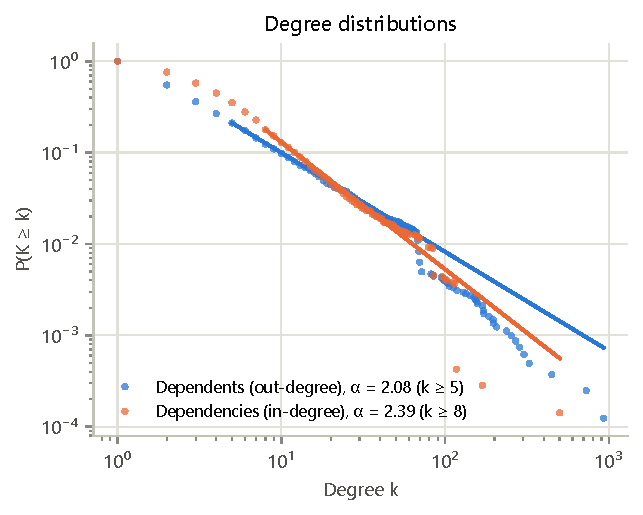
\includegraphics[width=0.55\linewidth]{fig1_degree_distribution.pdf}
\caption{Complementary cumulative degree distributions of the main graph, with discrete power-law fits
above $x_{\min}$. Dependents correspond to the contagion out-degree.}
\label{fig:degree}
\end{figure}

\section{Model}\label{sec:model}

\subsection{Contagion graph}
Let $G_{\text{dep}}=(V,E)$ contain an edge $u\to v$ whenever package $u$ depends on $v$. Malicious code
flows against this arrow: a compromised $v$ exposes every $u$ that installs it. Our contagion graph is
therefore the reversal $G=G_{\text{dep}}^{\top}$, with edges $v\to u$. Each node is susceptible (S),
infected (I) or recovered (R). Here \emph{infected} means that the package has published a malicious
version, and \emph{recovered} means that it has been patched, unpublished or protected.
\Cref{fig:model} shows both contagion channels.

\begin{figure}[t]
\centering
\begin{tikzpicture}[
  pkg/.style={draw, rounded corners=2pt, minimum width=1.25cm, minimum height=0.55cm, font=\small},
  inf/.style={pkg, fill=orange!25},
  dep/.style={-{Latex[length=2mm]}, thick},
  cred/.style={-{Latex[length=2mm]}, thick, dashed, blue!70!black},
  lab/.style={font=\scriptsize, midway, fill=white, inner sep=1pt}]
  \node[inf] (v) {$v$};
  \node[pkg, right=2.2cm of v] (u) {$u$};
  \node[pkg, below=0.9cm of u] (w1) {$w_1$};
  \node[pkg, right=0.4cm of w1] (w2) {$w_2$};
  \node[font=\small, right=0.15cm of w2] (dots) {$\cdots$};
  \node[draw, circle, inner sep=1pt, font=\small, above=0.6cm of $(u)!0.5!(w2)$, xshift=1.4cm] (m) {$m$};
  \draw[dep] (v) -- node[lab, above=2pt] {$\beta\, w_{\text{semver}}\, w_{\text{exec}}(u)$} (u);
  \draw[cred] (u) to[bend left=15] node[lab, above right=-1pt] {token, $\beta_m$} (m);
  \draw[cred] (m) -- (w1);
  \draw[cred] (m) -- (w2);
  \node[font=\scriptsize, below=0.25cm of w1, xshift=0.8cm] {republish $\leq$ cap packages of $m$};
  \begin{scope}[on background layer]
    \node[draw=gray!50, dashed, rounded corners, fit=(u)(w1)(w2)(dots)(m), inner sep=6pt,
          label={[font=\scriptsize, gray]above:maintainer $m$'s packages}] {};
  \end{scope}
\end{tikzpicture}
\caption{The two contagion channels. In the dependency channel (solid), compromised $v$ infects
dependent $u$ when $u$'s maintainer installs it and the injected install script runs. In the credential
channel (dashed), an infected package leaks its maintainer's token, and the worm republishes up to a
capped number of that maintainer's other packages.}
\label{fig:model}
\end{figure}

\subsection{Dependency channel}
In each discrete tick, every infected $v$ infects each susceptible successor $u$ independently with
probability
\begin{equation}
  \beta_{vu} = \min\bigl(1,\; \beta \cdot w_{\text{semver}}(v,u) \cdot w_{\text{exec}}(u) \cdot w_{\text{prov}}(u)\bigr).
  \label{eq:beta}
\end{equation}
The three weights are:
\begin{itemize}
  \item \textbf{SemVer weight.} $w_{\text{semver}}$ encodes how readily $u$'s constraint accepts an
        automatic malicious release: exact $0.05$, tilde $0.85$, caret and wildcard $1.0$.
  \item \textbf{Script execution.} The worm injects its own lifecycle script into every package it
        republishes, so every infected source carries the payload. What varies is the consumer:
        $w_{\text{exec}}(u)=0.1$ if $u$'s maintainers or CI block lifecycle scripts, and $1$ otherwise.
        The residual $0.1$ covers runtime execution paths. In the status quo we assume 10\% of
        packages block scripts, reflecting pnpm~$\geq$10, Bun and \texttt{--ignore-scripts} users. The
        blocking sets are nested across regimes. The original static formulation, which boosts packages
        that \emph{declare} install scripts, made script blocking ineffective by construction; we keep
        it only as a variant.
  \item \textbf{Provenance.} $w_{\text{prov}}(u)$ is a provenance factor applied in hardened regimes
        (\cref{sec:rq2}).
\end{itemize}

\subsection{Credential channel}
In each tick, every infected package leaks each of its not-yet-compromised maintainers' tokens with
probability $\beta_m$. A compromised maintainer has up to $c$ of their packages republished in the next
tick, chosen at random; packages with provenance are republished with probability $w_{\text{prov}}$.
The cap $c$ mirrors the observed limits of 20 (wave~1) and 100 (wave~2) packages per token.

\subsection{Recovery, interventions and metrics}
\paragraph{Recovery.} Infected packages recover with probability $\gamma$ per tick from the
\emph{detection tick} onward. Nobody patches a worm that has not yet been discovered. One tick
corresponds to one hour.

\paragraph{Interventions.} An intervention policy moves up to $B$ nodes per tick to R from the detection
tick onward. It can target infected nodes uniformly at random (\emph{random patching}) or in order of
contagion out-degree (\emph{hub patching}). Alternatively, a set of $K$ nodes is immunized at $t=0$, in
one of three ways:
\begin{itemize}
  \item \emph{firebreak}: highest betweenness;
  \item \emph{hub}: highest out-degree;
  \item \emph{acquaintance}: random neighbours of random nodes~\citep{cohen2003acquaintance}.
\end{itemize}

\paragraph{Metrics.} The final outbreak size $\Rinf$ is the fraction of packages \emph{ever} infected.
It excludes immunized and patched nodes, which would otherwise inflate $|R(\infty)|$ precisely when
defences work. We also report:
\begin{itemize}
  \item $T_{80}$: the time to infect 80\% of the patient zero's dependency-reachable set;
  \item $T_{90}$: the time to reach 90\% of a run's final size, i.e.\ the plateau;
  \item peak prevalence;
  \item infection-tree depth;
  \item the share of infections caused by the credential channel;
  \item the probability of a major outbreak ($\Rinf\geq5\%$).
\end{itemize}

\subsection{Simulation and statistics}
Each configuration is run 100 times (50 for the RQ2 grids). Run $i$ of a configuration uses child $i$
of a NumPy \pkg{SeedSequence}. Configurations that share a seed are therefore \emph{paired}: run $i$
gets the same patient-zero draw and random stream across strategies and regimes. Outbreak sizes are
bimodal, so we report percentile-bootstrap 95\% confidence intervals and give the probability of a major
outbreak separately from its size. Paired reductions use a paired bootstrap.

The engine is vectorised over a CSR representation of $G$, so 100 runs on the 10k graph take about one
second. We cross-validated it against NDlib's SIR model~\citep{rossetti2018ndlib}: with homogeneous
weights, mean outbreak sizes agree within sampling error.

\begin{table}[t]
\centering
\caption{Parameters. Ticks are hours. SH1 and SH2 values are calibrated in \cref{sec:calibration}.
Patching starts at the detection tick.}
\label{tab:params}
\begin{tabular}{llccc}
\toprule
Symbol & Meaning & Spec reference & SH1-calibrated & SH2-calibrated \\
\midrule
$\beta$ & dependency transmission & 0.15 & \CalOneBeta & \CalTwoBeta \\
$\beta_m$ & token leak per maintainer and tick & 0 & \CalOneBetaM & \CalTwoBetaM \\
$\gamma$ & patching rate after detection & 0.05 & \CalOneGamma & \CalTwoGamma \\
$c$ & packages republished per token & 20 & \CalOneCap & \CalTwoCap \\
$t_{\text{det}}$ & detection tick (h) & 0 & \CalOneDetect & \CalTwoDetect \\
\bottomrule
\end{tabular}
\end{table}

\section{Calibration and Empirical Validation}\label{sec:calibration}

\subsection{Incident data}
We compiled the packages compromised in both Shai-Hulud waves from public indicator lists and vendor
reports~\citep{stepsecurity2025shaihulud,socket2025shaihulud,wiz2025shaihulud2,datadog2025shaihulud2}.
This gives \ValOneListed{} packages for wave~1 and \ValTwoListed{} for wave~2. Publish timestamps come
from registry metadata, which survives takedown. Three facts from the incidents anchor the calibration:
\begin{enumerate}
  \item \textbf{Detection lag.} Wave~1 went about 24\,h from the first malicious publish to the first
        public signal. Wave~2 was flagged by automated feeds within minutes.
  \item \textbf{Plateau.} 90\% of the compromised versions had appeared 37\,h (wave~1) and 13.4\,h
        (wave~2) after the first publish.
  \item \textbf{Mechanism.} Most compromised packages were produced by stolen-token republishing.
        Publish bursts match the per-token caps, and only about 230 of the about 800 wave-2 packages have
        any dependents at all. We therefore target a credential-channel share of 75\%.
\end{enumerate}

\subsection{Calibration}
We grid-search $\beta\in[0.005,0.3]$, $\beta_m\in[0.005,0.5]$ and $\gamma\in[0.05,0.4]$ on the main graph,
with each wave's cap and detection tick fixed. Each configuration gets 40 runs, each from a uniformly
random patient zero. Plateau time and channel share are evaluated on major outbreaks only, since the
observed waves are by definition outbreaks that took off. The loss is the squared log-error of the
median $T_{90}$ plus the squared, scaled error of the channel share.

Both best fits lie inside the grid:
\begin{itemize}
  \item \textbf{SH1-calibrated:} $\beta=\CalOneBeta$, $\beta_m=\CalOneBetaM$, $\gamma=\CalOneGamma$,
        giving a plateau at $T_{90}=\CalOneTninety$\,h with \CalOneShare{} of infections via the
        credential channel.
  \item \textbf{SH2-calibrated:} $\beta=\CalTwoBeta$, $\beta_m=\CalTwoBetaM$, $\gamma=\CalTwoGamma$,
        giving $T_{90}=\CalTwoTninety$\,h and a credential share of \CalTwoShare.
\end{itemize}

The data constrain transmission well. Configurations within a loss tolerance of 0.1 of the optimum span
$\beta\in\CalOneBetaRange$ and $\beta_m\in\CalOneBetaMRange$ for wave~1, and $\beta\in\CalTwoBetaRange$
and $\beta_m\in\CalTwoBetaMRange$ for wave~2. They do not identify $\gamma$, since every value we tried
fits, nor the absolute outbreak size, since median major-outbreak sizes range over \CalOneSizeRange{}
packages for wave~1.

We therefore treat outbreak sizes in the high-impact core as \emph{projections}. They answer the
question ``what if a worm with Shai-Hulud's dynamics reached the core?'', not ``what did Shai-Hulud
do''.

\subsection{Validation of the channel structure}
If the credential channel dominates, victims should cluster by shared maintainer much more than by
dependency links. We fetched current registry metadata, never package contents, for
\ValOneN{} of the wave-1 and \ValTwoN{} of the wave-2 packages. We then compared them with random sets of
equal size drawn from the full closure (\cref{tab:validation}).

\begin{table}[t]
\centering
\caption{Clustering of real Shai-Hulud victims. A package counts as \emph{co-maintained} if it shares a
maintainer with another victim, and as \emph{dependency-linked} if it has an installed dependency edge to
another victim. The null is the mean over 200 random sets of equal size from the full closure. The last
column counts victims present in the full-closure graph.}
\label{tab:validation}
\begin{tabular}{lrrrrrr}
\toprule
 & & \multicolumn{2}{c}{Co-maintained} & \multicolumn{2}{c}{Dependency-linked} & In core \\
\cmidrule(lr){3-4}\cmidrule(lr){5-6}
Wave & $n$ & observed & null & observed & null & graph \\
\midrule
Shai-Hulud 1 & 189 & 98\% & 49\% & 32\% & 5\% & 2 \\
Shai-Hulud 2 & 732 & 95\% & 69\% & 23\% & 14\% & 7 \\
\bottomrule
\end{tabular}

\end{table}

The pattern is clear:
\begin{itemize}
  \item \ValOneCoMaint{} of wave-1 victims share a maintainer with another victim, against
        \ValOneCoMaintNull{} in the null. For wave~2 the figures are \ValTwoCoMaint{} and
        \ValTwoCoMaintNull.
  \item Installed dependency links are much rarer: \ValOneDepLinked{} and \ValTwoDepLinked{} of victims.
  \item Almost no victims belong to the high-impact core: \ValOneInFull{} wave-1 and \ValTwoInFull{}
        wave-2 packages appear in the full closure.
\end{itemize}

The null is drawn from the high-impact closure, where monorepo organisations inflate co-maintenance, so
the contrast is conservative. Taken together, the evidence shows that the real waves spread through
stolen tokens among the periphery's small maintainers. Our experiments ask what happens when such a worm
enters the core.

\section{Results}\label{sec:results}

All results in this section use the main graph and the script-blocking status quo, unless stated
otherwise.

\subsection{RQ1: Does the origin of an outbreak matter?}\label{sec:rq1}
We use four origin groups, each disjoint from the others:
\begin{itemize}
  \item \emph{hubs}: the ten packages with the most direct dependents;
  \item \emph{bridges}: the ten with the highest betweenness among the remaining packages;
  \item \emph{mid-tier}: ten packages at the median k-core;
  \item \emph{leaves}: ten packages in the bottom 20\% by contagion out-degree.
\end{itemize}
We start 100 outbreaks from each package in each group, under four parameter scenarios
(\cref{tab:rq1,fig:rq1}).

\begin{table}[t]
\centering
\caption{RQ1: mean final outbreak size $\Rinf$ with 95\% bootstrap CI, and in parentheses the
probability of a major outbreak ($\Rinf\geq5\%$), by patient-zero group. Each cell aggregates 1{,}000 runs.}
\label{tab:rq1}
\small
\begin{tabular}{lcccc}
\toprule
Scenario & Hub & Bridge & Mid-tier & Leaf \\
\midrule
Spec reference & 5.3\% [5.1\%, 5.4\%] (46\%) & 0.8\% [0.8\%, 0.9\%] (0\%) & 0.2\% [0.2\%, 0.2\%] (0\%) & 0.0\% [0.0\%, 0.0\%] (0\%) \\
Dependency only & 2.6\% [2.5\%, 2.7\%] (11\%) & 0.2\% [0.2\%, 0.3\%] (0\%) & 0.0\% [0.0\%, 0.0\%] (0\%) & 0.0\% [0.0\%, 0.0\%] (0\%) \\
SH1-calibrated & 55.8\% [55.6\%, 55.9\%] (100\%) & 48.7\% [48.0\%, 49.4\%] (95\%) & 31.8\% [30.2\%, 33.3\%] (63\%) & 19.6\% [18.1\%, 21.0\%] (40\%) \\
SH2-calibrated & 85.8\% [85.7\%, 85.8\%] (100\%) & 84.2\% [83.4\%, 84.9\%] (98\%) & 78.8\% [77.2\%, 80.2\%] (92\%) & 55.4\% [52.8\%, 57.8\%] (64\%) \\
\bottomrule
\end{tabular}

\end{table}

\begin{figure}[t]
\centering
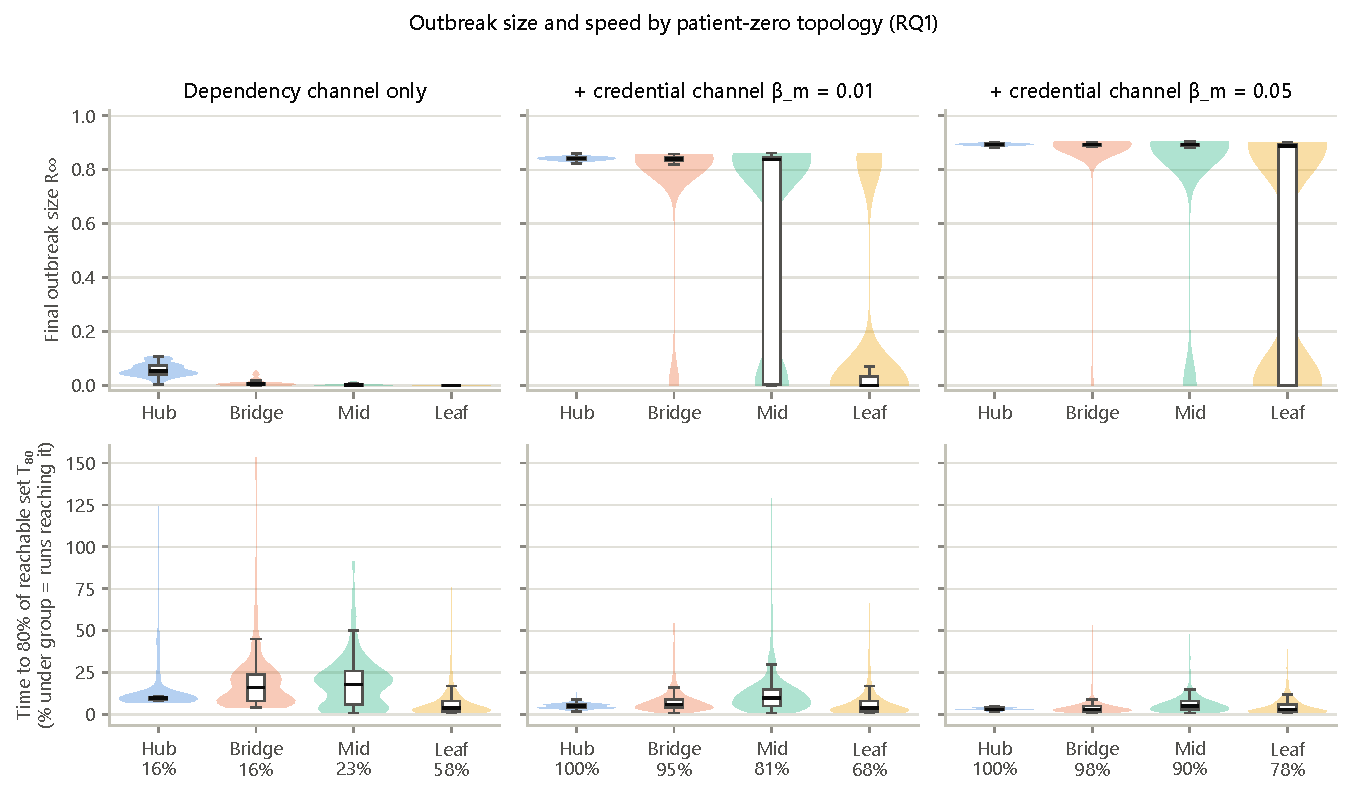
\includegraphics[width=\linewidth]{fig3_superspreader_comparison.pdf}
\caption{RQ1. Top: distributions of the final outbreak size $\Rinf$ by origin group and scenario. Bottom:
time to infect 80\% of the dependency-reachable set, for runs that reach it (the share of runs is shown
under each group).}
\label{fig:rq1}
\end{figure}

\paragraph{Dependency-only spread is bounded and hub-driven.}
In the spec-reference and dependency-only scenarios, outbreaks seeded at hubs reach \RQOneSpecRefHub{}
and \RQOneDepOnlyHub{} of the core, respectively. Outbreaks seeded at leaves essentially never spread.
Because the graph is nearly acyclic, an outbreak can only travel down the dependents of its origin, and
transmission is stochastic with $\beta<1$. A hub therefore reaches only a fraction of its static blast
radius before patching stops it. Topology matters strongly here, and the super-spreader hypothesis holds.

\paragraph{The credential channel erases most of the origin effect.}
With the SH1-calibrated credential channel:
\begin{itemize}
  \item hub-seeded outbreaks reach \RQOneShOneHub{} of the core;
  \item outbreaks seeded at leaves, which cannot spread at all through dependencies, still reach
        \RQOneShOneLeaf{} on average, with a major outbreak in \RQOneShOneLeafPmajor{} of runs.
\end{itemize}
Under SH2 parameters the corresponding figures are \RQOneShTwoHub{} and \RQOneShTwoLeaf. Between
\RQOneShOneLeafMaint{} and \RQOneShOneHubMaint{} of infections come through stolen tokens. Outbreak-size
distributions become strongly bimodal (\cref{fig:rq1}): an outbreak either dies out before a token leaks
or takes over most of the core. Origin topology mainly changes the \emph{probability} of take-off, not
the size of outbreaks that do take off. \Cref{fig:sir} shows the resulting epidemic curves.

\begin{figure}[t]
\centering
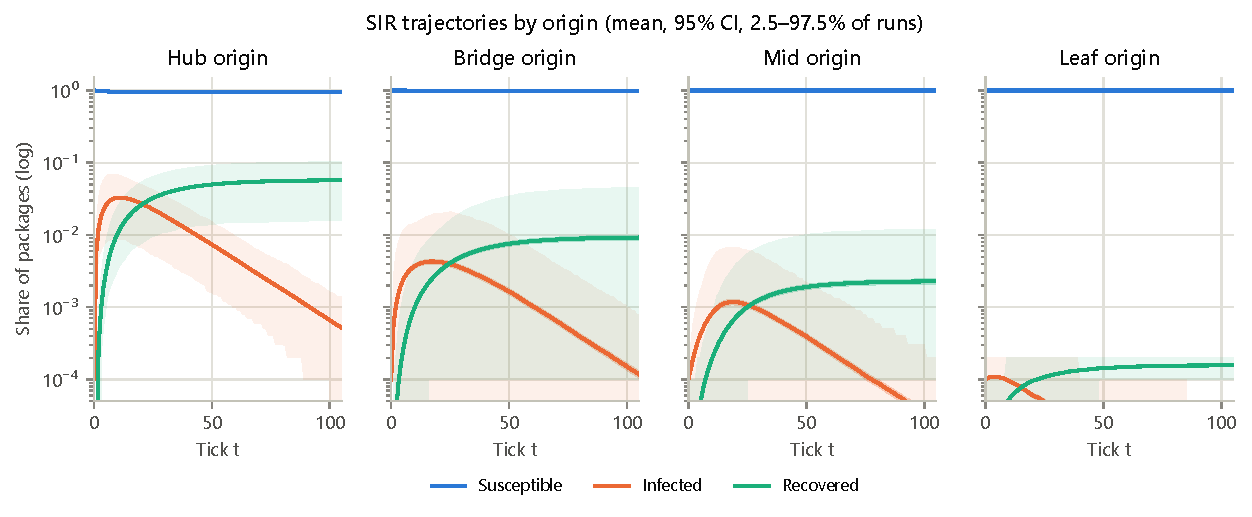
\includegraphics[width=\linewidth]{fig2_sir_epidemic_curves.pdf}
\caption{S/I/R trajectories (log scale) under SH1-calibrated parameters, by origin group: mean, 95\% CI
of the mean, and the 2.5--97.5\% envelope of runs. Patching starts at $t=24$\,h.}
\label{fig:sir}
\end{figure}

\subsection{RQ2: Which ecosystem regimes shift the threshold?}\label{sec:rq2}
We compare four regimes:
\begin{itemize}
  \item \emph{status quo}: the observed SemVer mix, with 10\% of packages blocking scripts;
  \item \emph{strict lockfile}: loose constraints pinned until 80\% of edges are exact;
  \item \emph{scripts disabled}: 70\% of packages block lifecycle scripts;
  \item \emph{hardened}: strict lockfiles, scripts disabled and trusted publishing on the top 5\% of hubs.
        In the hardened regime, stolen-token publishes to these hubs succeed with probability 0.1.
\end{itemize}
For each regime we sweep a 13$\times$5 grid of $(\beta,\gamma)$ with hub-seeded outbreaks and estimate
the critical $\beta_c$ at which the mean $\Rinf$ reaches 5\% (\cref{tab:rq2,fig:rq2}).

\begin{table}[t]
\centering
\caption{RQ2, dependency channel only ($\beta_m=0$): empirical critical transmission rate $\beta_c$ at
which mean $\Rinf$ reaches 5\%. ``none'' means that no grid value up to $\beta=1$ produced a major
outbreak.}
\label{tab:rq2}
\begin{tabular}{lccccc}
\toprule
Regime & $\gamma=0.02$ & $\gamma=0.05$ & $\gamma=0.10$ & $\gamma=0.20$ & $\gamma=0.40$ \\
\midrule
Status quo & 0.045 & 0.125 & 0.274 & 0.363 & 0.499 \\
Strict lockfile & 0.514 & 0.917 & none & none & none \\
Scripts disabled & 0.279 & 0.642 & none & none & none \\
Hardened & none & none & none & none & none \\
\bottomrule
\end{tabular}

\end{table}

\begin{figure}[t]
\centering
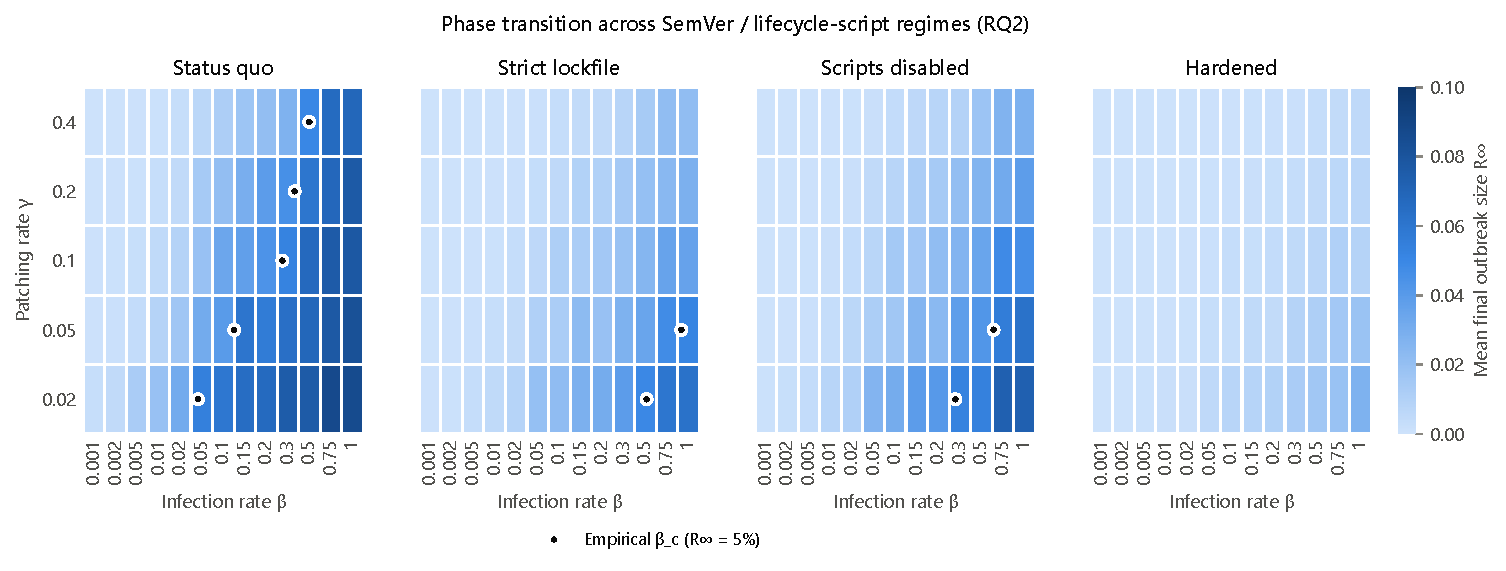
\includegraphics[width=\linewidth]{fig4_semver_phase_transition.pdf}
\caption{RQ2: mean $\Rinf$ over the $(\beta,\gamma)$ grid for each regime, dependency channel only.
Markers show the empirical $\beta_c$.}
\label{fig:rq2}
\end{figure}

\paragraph{Without stolen tokens, dependency-side hardening works.}
At $\gamma=\RQTwoGammaLow$ the status quo has $\beta_c=\RQTwoBetaSQ$. Strict lockfiles raise it to
\RQTwoBetaSL{} (about \RQTwoLockFactor$\times$), and blocking scripts on 70\% of packages raises it to
\RQTwoBetaSD{} (about \RQTwoScriptsFactor$\times$). The hardened regime never produces a major outbreak.
The spectral prediction $\tau_c=1/\lambda_{\max}=\RQTwoTauTheory$ lies far from these empirical
thresholds. This is expected for SIR on a nearly acyclic directed graph, where $1/\lambda_{\max}$ is only
a lower bound that is set by small monorepo cycles~\citep{li2013directed}.

\paragraph{With stolen tokens, the dependency threshold collapses.}
With the calibrated credential rates $\beta_m\in\{\CalOneBetaM,\CalTwoBetaM\}$, the estimated $\beta_c$
falls to the bottom of our grid (0.001) in \RQTwoCredCollapsed{} of regime--$\gamma$ combinations. The
credential channel alone sustains the epidemic, so the relevant threshold is in $\beta_m$, not $\beta$.
\Cref{tab:rq2b} reports the critical $\beta_m$ per regime at the SH1 transmission rate.
\RQTwoBDone

\begin{table}[t]
\centering
\caption{RQ2b: empirical critical token-leak rate $\beta_{m,c}$ per regime at $\beta=\CalOneBeta$.}
\label{tab:rq2b}
\begin{tabular}{lccccc}
\toprule
Regime & $\gamma=0.02$ & $\gamma=0.05$ & $\gamma=0.10$ & $\gamma=0.20$ & $\gamma=0.40$ \\
\midrule
Status quo & $\leq$0.001 & 0.001 & 0.002 & 0.008 & 0.020 \\
Strict lockfile & 0.001 & 0.002 & 0.005 & 0.015 & 0.031 \\
Scripts disabled & $\leq$0.001 & 0.001 & 0.004 & 0.012 & 0.028 \\
Hardened & 0.002 & 0.006 & 0.015 & 0.038 & 0.087 \\
\bottomrule
\end{tabular}

\end{table}

\subsection{RQ3: Patch reactively or immunize proactively?}\label{sec:rq3}
Outbreaks are seeded at hubs under SH1-calibrated parameters. Both reactive patching and natural
recovery begin only at the detection delay $t_{\text{det}}\in\{1,6,12,24,48\}$\,h.
\begin{itemize}
  \item Reactive policies treat up to $B$ packages per hour, either hubs first or at random.
  \item Proactive policies immunize $K$ packages at $t=0$, choosing them by betweenness, by degree or by
        acquaintance sampling.
\end{itemize}
To compare at equal cost, $K$ is set to the mean number of packages that hub patching treats at the same
$B$ and delay. \Cref{tab:rq3} reports paired reductions in $\Rinf$ at $B=\RQThreeBudget$ packages per hour
(\RQThreeBudgetPct{} of the graph), and \cref{fig:rq3} shows all budgets.

\begin{table}[t]
\centering
\caption{RQ3: share of the no-intervention outbreak prevented (paired, mean over 100 runs) at
$B=\RQThreeBudget$ per hour, by detection delay. The last row gives the no-intervention $\Rinf$, which
grows with the delay because natural patching also waits for detection.}
\label{tab:rq3}
\begin{tabular}{lccccc}
\toprule
Strategy & 1\,h & 6\,h & 12\,h & 24\,h & 48\,h \\
\midrule
Hub patching & 100\% & 90\% & 52\% & 13\% & 3\% \\
Random patching & 100\% & 76\% & 23\% & 5\% & 1\% \\
Firebreak (betweenness) & 3\% & 13\% & 27\% & 29\% & 26\% \\
Hub immunization & 6\% & 23\% & 38\% & 42\% & 40\% \\
Acquaintance & 3\% & 17\% & 32\% & 35\% & 34\% \\
\midrule
No intervention $R_\infty$ & 47\% & 48\% & 49\% & 55\% & 68\% \\
\bottomrule
\end{tabular}

\end{table}

\begin{figure}[t]
\centering
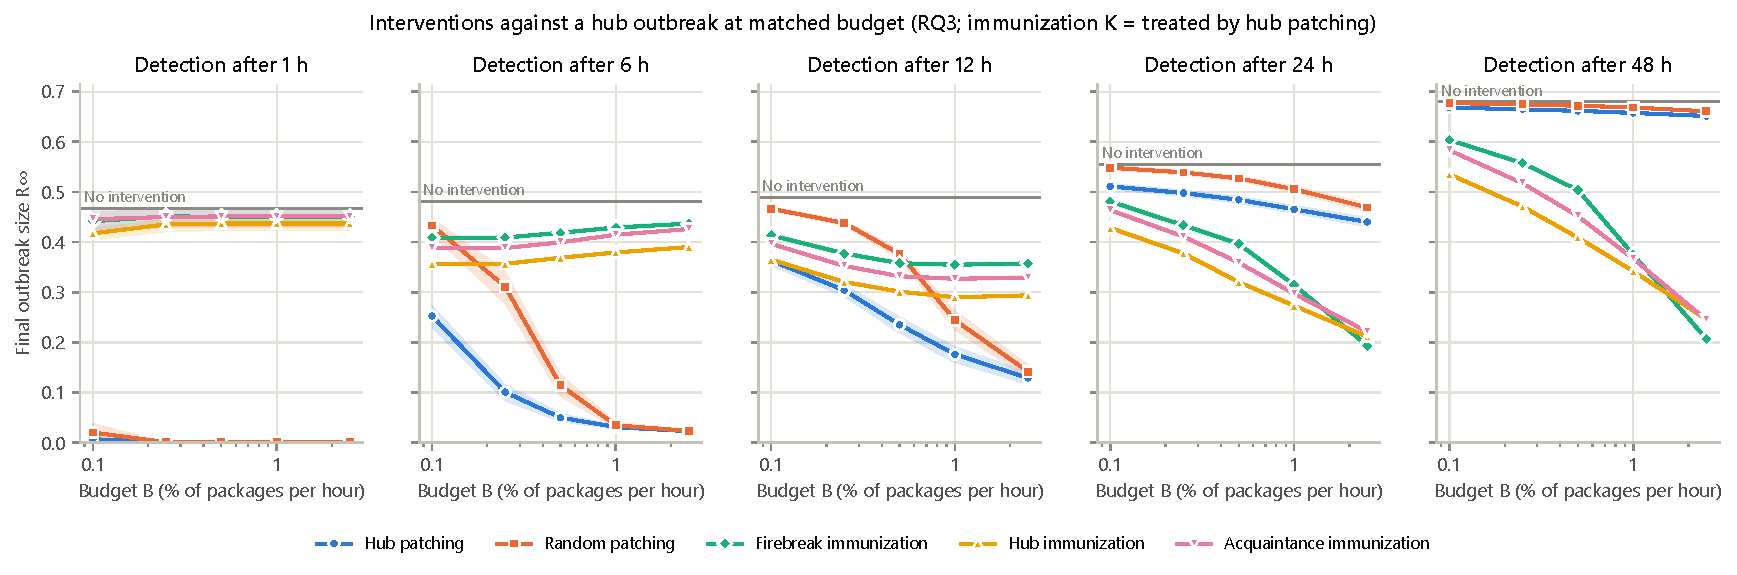
\includegraphics[width=\linewidth]{fig5_firebreak_immunization.pdf}
\caption{RQ3: final outbreak size against the intervention budget $B$ (95\% CI), by detection delay.
Proactive strategies immunize the same total number of packages that hub patching treats.}
\label{fig:rq3}
\end{figure}

\paragraph{Reactive patching works only with fast detection.}
Detected within an hour, the outbreak is almost fully contained by either reactive policy (hub patching
prevents \RQThreeHubPatchingOne). Its value drops quickly with delay: \RQThreeHubPatchingSix{} prevented
at 6\,h, \RQThreeHubPatchingTwelve{} at 12\,h, and only \RQThreeHubPatchingTwentyFour{} at 24\,h, which
was the lag of wave~1.

\paragraph{Proactive immunization holds up, and degree beats betweenness.}
Immunizing high-degree packages at the same total cost prevents \RQThreeHubImmunizationTwelve{} at 12\,h
and \RQThreeHubImmunizationTwentyFour{} at 24\,h. The two approaches cross over between 12 and 24\,h of
delay: reactive patching is still ahead at 12\,h, and proactive immunization is well ahead at 24\,h and
48\,h. Acquaintance immunization, which needs no global knowledge, comes close
(\RQThreeAcquaintanceTwentyFour{} at 24\,h).

Betweenness ``firebreaks'' are weaker under the credential channel (\RQThreeFirebreakBetweennessTwentyFour{}
at 24\,h). A plausible explanation is that betweenness targets packages that cut dependency paths,
whereas under the credential channel most infections bypass those paths through stolen tokens; we have
not tested this mechanism directly. Betweenness is a heuristic; optimized immunization sets could do
better~\citep{schneider2011limited}. Our claim is therefore limited to the comparison with degree-based
and random strategies at matched cost.

\section{Robustness}\label{sec:robustness}

\paragraph{Synthetic ensemble.}
Across \SynSeeds{} synthetic scale-free graphs (DAGs with $n=\SynN$) under SH1 parameters, hub-seeded
outbreaks reach $\SynHubMean\pm\SynHubSD$ and leaf-seeded ones $\SynLeafMean\pm\SynLeafSD$ (mean
$\pm$ s.d.\ across seeds). Hub immunization is the best RQ3 strategy at 24\,h delay and maximum budget
in \SynRQThreeBestCount{} graphs. The qualitative RQ1 and RQ3 conclusions therefore do not depend on the
particular structure of the npm crawl. The synthetic graphs differ from npm in the size of the credential
effect: leaves reach much less, because synthetic maintainer portfolios are smaller and assigned
independently of the topology.

\paragraph{Sample size and null models.}
\Cref{tab:robustness} repeats the key quantities on three graph variants:
\begin{itemize}
  \item the 5k sample;
  \item the full 14{,}624-package closure;
  \item five degree-preserving rewirings of the main graph~\citep{maslov2002specificity}. These keep every
        package's in- and out-degree and the SemVer mix, but randomise who depends on whom.
\end{itemize}
The rewirings keep maintainer ownership fixed, so they separate the role of dependency structure from
that of the credential channel.

\begin{table}[t]
\centering
\caption{Robustness of the key quantities across graph variants. $\Rinf$ values are means over 1{,}000
runs per origin group.}
\label{tab:robustness}
\small
\begin{tabular}{lcccl}
\toprule
 & Hub $R_\infty$ & Hub $R_\infty$ & Leaf $R_\infty$ & Best RQ3 strategy \\
Graph & (dep.\ only) & (SH1) & (SH1) & (24\,h, max.\ budget) \\
\midrule
npm 5k & 2.3\% & 55.7\% & 22.4\% & Hub immunization \\
npm 10k (main) & 2.6\% & 55.8\% & 19.6\% & Firebreak (betweenness) \\
npm full closure & 2.2\% & 51.7\% & 7.8\% & Firebreak (betweenness) \\
null model 0 & 8.1\% & 64.2\% & 31.8\% & Acquaintance \\
null model 1 & \multicolumn{4}{c}{\textbf{[pending]}} \\
null model 2 & \multicolumn{4}{c}{\textbf{[pending]}} \\
null model 3 & \multicolumn{4}{c}{\textbf{[pending]}} \\
null model 4 & \multicolumn{4}{c}{\textbf{[pending]}} \\
\bottomrule
\end{tabular}

\end{table}

Three patterns stand out in \cref{tab:robustness}:
\begin{itemize}
  \item \textbf{npm's wiring dampens spread.} The \NullCount{} rewired graphs produce \emph{larger}
        outbreaks than the real one. Dependency-only hub outbreaks reach
        \NullDepHubMin--\NullDepHubMax{} instead of \RQOneDepOnlyHub, and SH1 leaf outbreaks reach
        \NullLeafMin--\NullLeafMax{} instead of \RQOneShOneLeaf. Random rewiring destroys npm's layered,
        nearly acyclic structure and creates cycles, so the real topology is protective relative to its
        degree sequence alone.
  \item \textbf{The leaf effect is a share of the graph.} SH1 leaf outbreaks reach \SizeFiveLeafShOne{},
        \SizeMainLeafShOne{} and \SizeFullLeafShOne{} of the 5k, 10k and full-closure graphs. In absolute terms that is between roughly 1{,}100 and 2{,}000 packages, so the
        share does not scale simply with graph size. We therefore report the leaf effect as a range
        rather than a single figure.
  \item \textbf{The RQ3 ranking is stable.} Proactive immunization beats reactive patching at a 24\,h
        delay on every variant. Which proactive heuristic is best at the largest budget varies between
        graphs (degree, betweenness or acquaintance), consistent with the convergence of the strategies
        at large $K$ in \cref{sec:rq3}.
\end{itemize}

\paragraph{Parameter sensitivity.}
Around the SH1 calibration (50 runs per setting) we vary $\beta\in\{0.01,0.02,0.05\}$ and $\gamma\in\{0.05,0.1,0.2\}$. The
conclusions hold across all of them:
\begin{itemize}
  \item a proactive strategy is the best RQ3 response at 24\,h delay and the largest budget in
        \SensProactiveBest{} settings;
  \item at $B=50$ per hour, hub immunization beats hub patching in \SensImmBeatsPatch{} settings and
        betweenness immunization in \SensDegreeBeatsFirebreak;
  \item the hub-to-leaf ratio of $\Rinf$ stays between \SensHubLeafMin{} and \SensHubLeafMax, so
        leaf-started outbreaks remain substantial whenever tokens can be stolen.
\end{itemize}

\section{Discussion}\label{sec:discussion}

\paragraph{Implications for defenders.}
Our results point to a clear order of priorities.
\begin{enumerate}
  \item \textbf{Credentials first.} The credential channel turns a bounded, hub-dependent process into
        one that can take over the core from almost any origin (RQ1). It also removes the epidemic
        threshold that dependency-side defences create (RQ2). Measures that break this channel therefore
        address the mechanism that actually drove both Shai-Hulud waves: short-lived and scoped tokens,
        trusted publishing that makes stolen tokens useless, and caps or rate limits on publishing from a
        single credential.
  \item \textbf{Then dependency hardening.} Lockfiles and blocking lifecycle scripts are still valuable.
        They raise the dependency-channel threshold by roughly an order of magnitude, and script blocking
        directly stops the install-time execution that harvests tokens. However, they are not sufficient
        while tokens remain stealable.
  \item \textbf{Proactive protection over reactive patching.} With limited response capacity and
        detection lags of a day, protecting the most-depended-upon packages in advance beats chasing
        infected ones. At realistic budgets degree is a better target than betweenness; at very large
        budgets the two converge.
\end{enumerate}
Lockfiles have a known cost: they slow the uptake of security fixes~\citep{pinckney2023semver}. And as
the s1ngularity and Mini Shai-Hulud incidents show, trusted publishing does not protect against a
compromised CI pipeline~\citep{wiz2025singularity,unit422026npmlandscape}.

\paragraph{Limitations.}
\begin{itemize}
  \item \textbf{Scope of the graph.} Our graph is the high-impact core, not all of npm. The real waves
        mostly struck peripheral packages (\cref{sec:calibration}), so absolute outbreak sizes in the
        core are projections. Calibration identifies dynamics (timescales and channel shares), not size.
  \item \textbf{Upper-bound assumptions.} The credential channel assumes that every infected package
        can leak its maintainers' tokens. Real leakage depends on whether a token was present on the
        infected machine, so our $\beta_m$ absorbs this probability.
  \item \textbf{Current metadata.} Maintainer lists and dependencies were fetched in 2026, not as they
        were at the time of the incidents.
  \item \textbf{Assumed adoption shares.} The shares of packages that block scripts (10\% and 70\%) are
        assumptions; we found no reliable measurement of them.
  \item \textbf{Static immunization.} Our immunization sets are static. Recalculated betweenness or
        optimized sets could perform better~\citep{holme2002attack,schneider2011limited}.
  \item \textbf{Remaining data quality.} A 17-package, low-density cluster of oddly named packages
        remains in the full closure below our spam threshold.
\end{itemize}

\paragraph{Ethics.}
We never downloaded, installed or executed compromised packages. Validation uses registry metadata and
public indicator lists only.

\section{Conclusion}\label{sec:conclusion}

We modelled self-propagating npm worms as a two-channel SIR epidemic and calibrated it to the two
Shai-Hulud waves. We validated its structure against the real victims, who cluster by shared maintainer
rather than by dependency links. We then used the model to evaluate where outbreaks start, which
ecosystem regimes change the epidemic threshold, and how to spend a limited response budget.

Dependency topology alone confines outbreaks to the dependents of a few hubs, and dependency-side
hardening raises that bound further. Stolen publish tokens remove it: with Shai-Hulud-like dynamics, a
worm that enters the high-impact core from an obscure leaf package can reach a large part of it, and
reactive patching after a day's delay barely helps. Breaking the credential channel, and proactively
protecting the most-depended-upon packages, are the most effective measures against the next worm.


\bibliographystyle{plainnat}
\bibliography{../docs/references}

\end{document}
